\documentclass[10pt]{beamer}

% Tema Limpo e Profissional
\usetheme{Madrid}
\usecolortheme{whale}

% Pacotes Essenciais
\usepackage[utf8]{inputenc}
\usepackage[portuguese]{babel}
\usepackage{graphicx}
\usepackage{booktabs}
\usepackage{amsmath}
\usepackage{amssymb}
\usepackage{listings}
\usepackage{xcolor}
\usepackage{tikz}

% Configuracoes de Codigo (Python)
\lstset{
    language=Python,
    basicstyle=\ttfamily\tiny,
    keywordstyle=\color{blue},
    stringstyle=\color{red},
    commentstyle=\color{green!60!black},
    breaklines=true,
    showstringspaces=false
}

% Metadados com Prevencao de Avisos de Metadados PDF
\title[ADS - Aula 14]{Regressão Linear Simples}
\subtitle{Da Reta em Unidades Padrão à Inferência Estatística}
\author[ADS - IFCE]{Tecnologia em Análise e Desenvolvimento de Sistemas\texorpdfstring{\\ \small{Ciência de Dados / Estatística Computacional}}{}}
\institute[IFCE]{Instituto Federal do Ceará -- Campus Tauá \\ Tecnologia em Análise e Desenvolvimento de Sistemas}
\date{\today}

\begin{document}

\begin{frame}
    \titlepage
\end{frame}

\begin{frame}{Sumário da Aula}
    \tableofcontents
\end{frame}

% Blocos Modulares de Slides
\section{A Reta de Regressão e a Função de Perda}

\begin{frame}{Como Predizer $Y$ a Partir de $X$?}
    \begin{columns}
        \begin{column}{0.5\textwidth}
            \textbf{Abordagem Local (Média Condicional):}
            \begin{itemize}
                \item Agrupamos os dados em janelas verticais estreitas no eixo $X$.
                \item Calculamos a média amostral da variável $Y$ para cada janela.
                \item Funciona bem se houver abundância de dados em todos os intervalos de $X$.
            \end{itemize}
        \end{column}
        \begin{column}{0.5\textwidth}
            \textbf{Abordagem Global (Modelo Linear):}
            \begin{itemize}
                \item E se as janelas tiverem poucos dados (esparsa amostragem)?
                \item Buscamos uma reta global contínua que descreva a tendência geral.
                \item Esta linha reta é a chamada \textbf{Reta de Regressão}.
            \end{itemize}
        \end{column}
    \end{columns}
\end{frame}

\begin{frame}{Reta em Unidades Padrão (Z-Scores)}
    \begin{itemize}
        \item Definimos Z-score (unidades padrão) de uma variável como:
        $$x_{su} = \frac{x_i - \bar{X}}{s_x}, \quad y_{su} = \frac{y_i - \bar{Y}}{s_y}$$
        \item Onde $\bar{X}, \bar{Y}$ são as \textbf{Médias Amostrais} e $s_x, s_y$ são os \textbf{Desvios Padrão Amostrais}.
        \item Em unidades padrão, a reta de regressão assume uma forma extremamente elegante:
        $$\hat{y}_{su} = r \cdot x_{su}$$
        \item Características:
        \begin{itemize}
            \item Sempre cruza a origem das coordenadas $(0, 0)$.
            \item A inclinação (slope) da reta é exatamente o \textbf{Coeficiente de Correlação de Pearson} ($r$).
        \end{itemize}
    \end{itemize}
\end{frame}

\begin{frame}{Considere o Gráfico ao Lado}
    \begin{columns}
        \begin{column}{0.5\textwidth}
            \textbf{Sintético}
            \begin{itemize}
                \item A linha vermelha é a linha de 45 graus.
                \item \textbf{Qual é o valor do Coeficiente Angular ($\beta$)?}
            \end{itemize}
            \vspace{0.4cm}
            \centering
            \begin{tikzpicture}[scale=1.3]
                \draw[->,>=stealth,thick] (0,0) -- (2.2,0) node[below] {$\Delta x$};
                \draw[->,>=stealth,thick] (0,0) -- (0,2.2) node[left] {};
                \draw[very thick] (0,0) -- (2,2) node[above right] {$y = \beta x + \alpha$};
                \draw[dashed] (2,0) -- (2,2) node[midway,right] {$\Delta y$};
            \end{tikzpicture}
        \end{column}
        \begin{column}{0.5\textwidth}
            \centering
            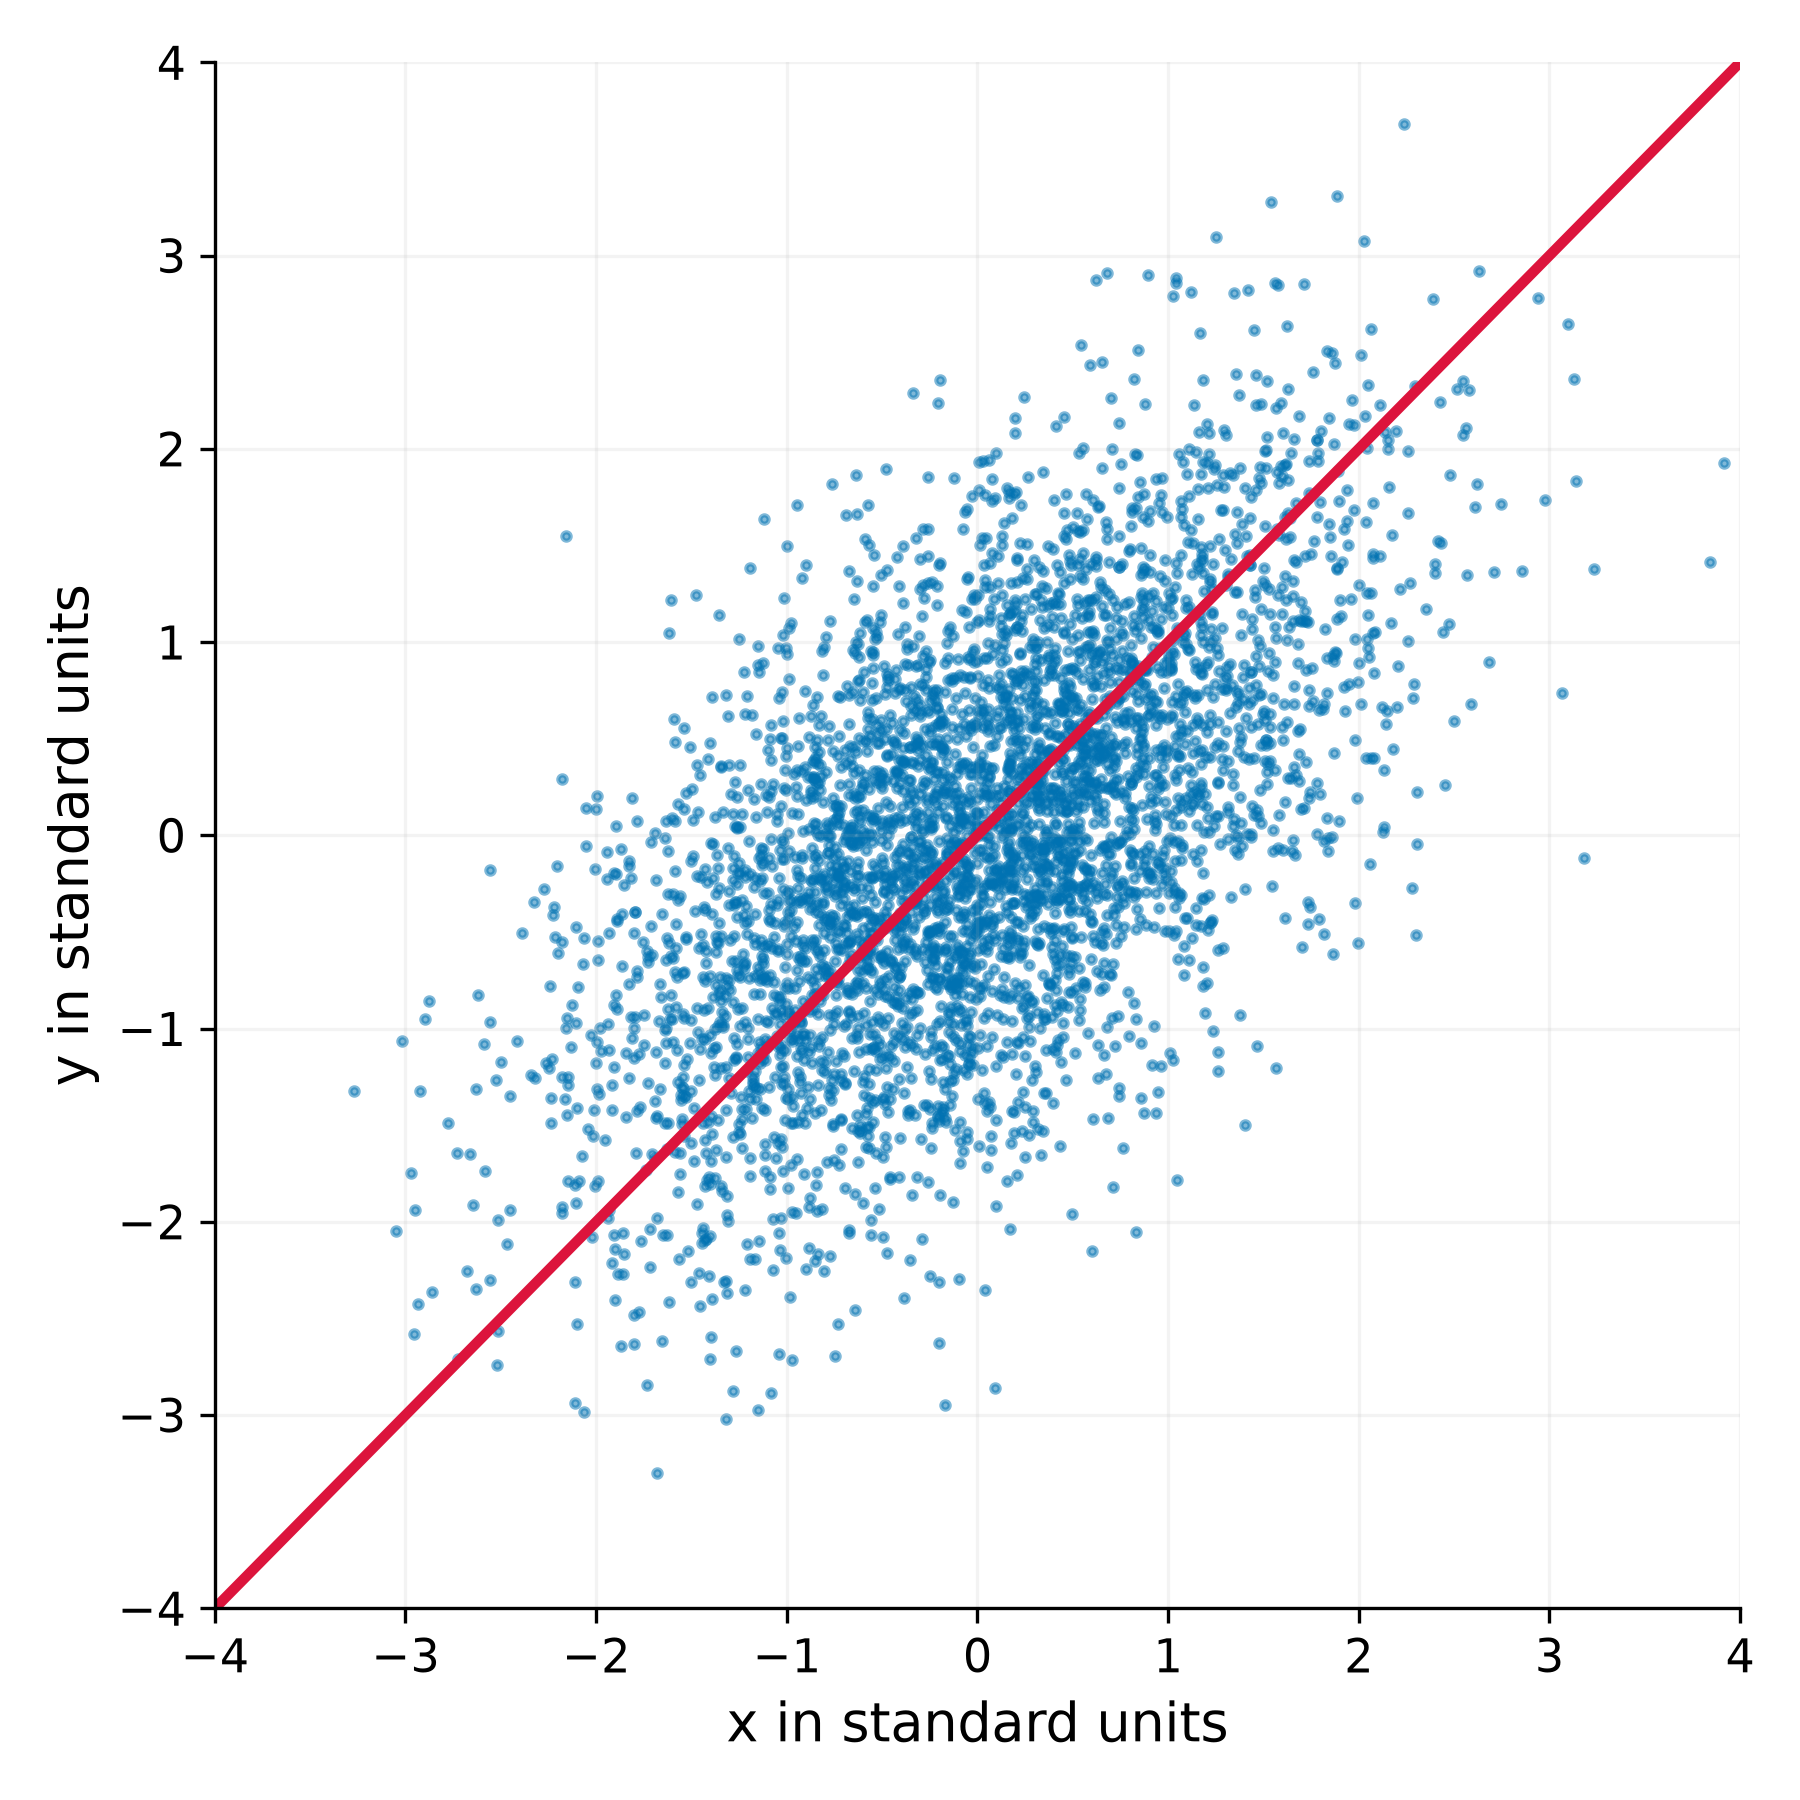
\includegraphics[width=0.95\textwidth]{grafico_linha_45.png}
        \end{column}
    \end{columns}
\end{frame}

\begin{frame}{O Efeito de Regressão (Regressão à Média)}
    \begin{itemize}
        \item Como $|r| \leq 1$, a inclinação da reta é menor ou igual a 1.
        \item \textbf{Efeito de Regressão:} A estimativa de $Y$ (em unidades padrão) estará sempre mais próxima da média do que o valor observado de $X$ (em unidades padrão).
        \item \textbf{Explicação Física:}
        \begin{itemize}
            \item Se um indivíduo apresenta uma medida extrema de $X$ (ex: $2$ desvios padrões acima da média), sua predição correspondente $\hat{Y}$ será de apenas $2 \cdot r$ desvios padrões acima da média.
            \item O fenômeno foi observado por Francis Galton em estudos de hereditariedade (pais muito altos tendem a ter filhos ligeiramente mais baixos que os pais, aproximando-se da média populacional).
        \end{itemize}
    \end{itemize}
\end{frame}

\begin{frame}{Erro de Estimativa e Função de Perda}
    \begin{itemize}
        \item Para qualquer reta de predição ajustada, existirá um \textbf{Erro de Estimativa} (ou Resíduo) para cada ponto:
        $$e_i = y_i - \hat{y}_i$$
        \item Como mensurar a qualidade de ajuste global do modelo?
        \item Definimos a \textbf{Função de Perda} (Loss Function) como a \textbf{Raiz do Erro Quadrático Médio} ($RMSE$):
        $$RMSE = \sqrt{\frac{1}{N} \sum_{i=1}^N (y_i - \hat{y}_i)^2}$$
        \item Onde $N$ representa o \textbf{Tamanho da Amostra}.
        \item Nosso objetivo estatístico é encontrar a reta que minimiza o valor de $RMSE$.
    \end{itemize}
\end{frame}

\begin{frame}{O Método dos Mínimos Quadrados (Least Squares)}
    \begin{itemize}
        \item O \textbf{Método dos Mínimos Quadrados Ordinários} ($OLS$) consiste em achar os parâmetros da reta que minimizam a soma dos erros quadrados de predição.
        \item Em unidades padrão, buscamos o slope $\beta_{su}$ da reta $\hat{y}_{su} = \beta_{su} \cdot x_{su}$ que minimize:
        $$L(\beta_{su}) = \frac{1}{N} \sum_{i=1}^N (y_{i,su} - \beta_{su} \cdot x_{i,su})^2$$
        \item Derivando em relação a $\beta_{su}$ e igualando a zero, prova-se analiticamente que:
        $$\beta_{su} = \frac{1}{N} \sum_{i=1}^N x_{i,su} \cdot y_{i,su} = r$$
        \item \textbf{Conclusão:} A reta de regressão em unidades padrão é a melhor reta no sentido dos mínimos quadrados.
    \end{itemize}
\end{frame}

\begin{frame}[fragile]{Exemplo Pareado: Otimização Computacional}
    \begin{block}{Minimizando o RMSE numericamente com SciPy}
\begin{lstlisting}
import numpy as np
from scipy.optimize import minimize
from scipy import stats

# Dados originais de exemplo
x = np.array([84.2, 88.1, 91.3, 85.0, 93.4])
y = np.array([89.1, 93.2, 94.5, 90.0, 97.2])

# Z-normalizacao (Unidades Padrao)
x_su = (x - np.mean(x)) / np.std(x, ddof=1)
y_su = (y - np.mean(y)) / np.std(y, ddof=1)

# Funcao de perda: RMSE
def calcular_rmse(beta, x_data, y_data):
    pred = beta[0] * x_data
    return np.sqrt(np.mean((y_data - pred) ** 2))

# Minimizacao numerica da perda
chute = [0.0]
res = minimize(calcular_rmse, chute, method='BFGS')
beta_otimizado = res.x[0]
r_analitico, _ = stats.pearsonr(x, y)

print(f"Beta Otimizado (RMSE): {beta_otimizado:.6f}")
print(f"Pearson r (Analitico): {r_analitico:.6f}")
\end{lstlisting}
    \end{block}
\end{frame}

\section{Regressão nas Unidades dos Dados, Diagnósticos e Qualidade}

\begin{frame}{A Reta nas Unidades Originais}
    \begin{itemize}
        \item Desfazendo a Z-normalização, chegamos à equação clássica da reta:
        $$\hat{y} = \beta X + \alpha$$
        \item \textbf{Fórmula do Coeficiente Angular (Slope $\beta$):}
        $$\beta = r \cdot \frac{s_y}{s_x}$$
        \item \textbf{Fórmula do Coeficiente Linear (Intercepto $\alpha$):}
        $$\alpha = \bar{Y} - \beta \bar{X}$$
        \item \textbf{Interpretação Prática:}
        \begin{itemize}
            \item \textbf{Slope} ($\beta$): Para cada acréscimo de uma unidade física em $X$, a predição $\hat{Y}$ aumenta em $\beta$ unidades físicas de $Y$.
            \item \textbf{Intercepto} ($\alpha$): Representa a predição para $Y$ caso a variável preditora $X$ assuma o valor zero (deve-se tomar cuidado com a extrapolação fora do domínio amostral).
        \end{itemize}
    \end{itemize}
\end{frame}

\begin{frame}{Qualidade do Ajuste: Coeficiente de Determinação}
    \begin{itemize}
        \item O \textbf{Coeficiente de Determinação} ($R^2$) indica a proporção da variabilidade da variável resposta $Y$ que é explicada pelo modelo linear:
        $$R^2 = 1 - \frac{\sum_{i=1}^N (y_i - \hat{y}_i)^2}{\sum_{i=1}^N (y_i - \bar{Y})^2}$$
        \item \textbf{Propriedades de $R^2$:}
        \begin{itemize}
            \item Na regressão linear simples, vale exatamente o quadrado do coeficiente de Pearson ($R^2 = r^2$).
            \item Varia no intervalo $[0, 1]$ para regressões de mínimos quadrados comuns.
            \item Exemplo: $R^2 = 0.65 \implies 65\%$ da variação dos dados de Y é explicada linearmente em relação a X.
        \end{itemize}
    \end{itemize}
\end{frame}

\begin{frame}{Diagnósticos Visuais de Regressão}
    \begin{itemize}
        \item O \textbf{Gráfico de Resíduos} (Residual Plot) é a principal ferramenta de diagnóstico visual. Consiste em plotar os resíduos $e_i = y_i - \hat{y}_i$ contra o preditor $x_i$.
        \item \textbf{Suposição de Homocedasticidade:} A variabilidade dos resíduos deve ser constante ao longo de todo o eixo X.
        \item \textbf{Padrões Indesejados a Detectar:}
        \begin{enumerate}
            \item \textbf{Não-Linearidade:} Resíduos formam curvas (ex: padrão em U). Sugere necessidade de transformações ou modelos não-lineares.
            \item \textbf{Heterocedasticidade:} Resíduos apresentam-se em forma de funil (dispersão aumenta com X). Afeta a validade das inferências estatísticas clássicas.
        \end{enumerate}
    \end{itemize}
\end{frame}

\begin{frame}{Diagnósticos Visuais: Homocedasticidade}
    \begin{columns}
        \begin{column}{0.5\textwidth}
            \textbf{Caso 1: Homocedástico (Ideal)}
            \begin{itemize}
                \item Os resíduos apresentam-se dispersos de forma aleatória em torno da linha zero.
                \item A variabilidade (dispersão vertical) é constante ao longo de todo o eixo $X$.
                \item Esta é a situação ideal que valida as inferências e testes de hipóteses clássicos.
            \end{itemize}
        \end{column}
        \begin{column}{0.5\textwidth}
            \centering
            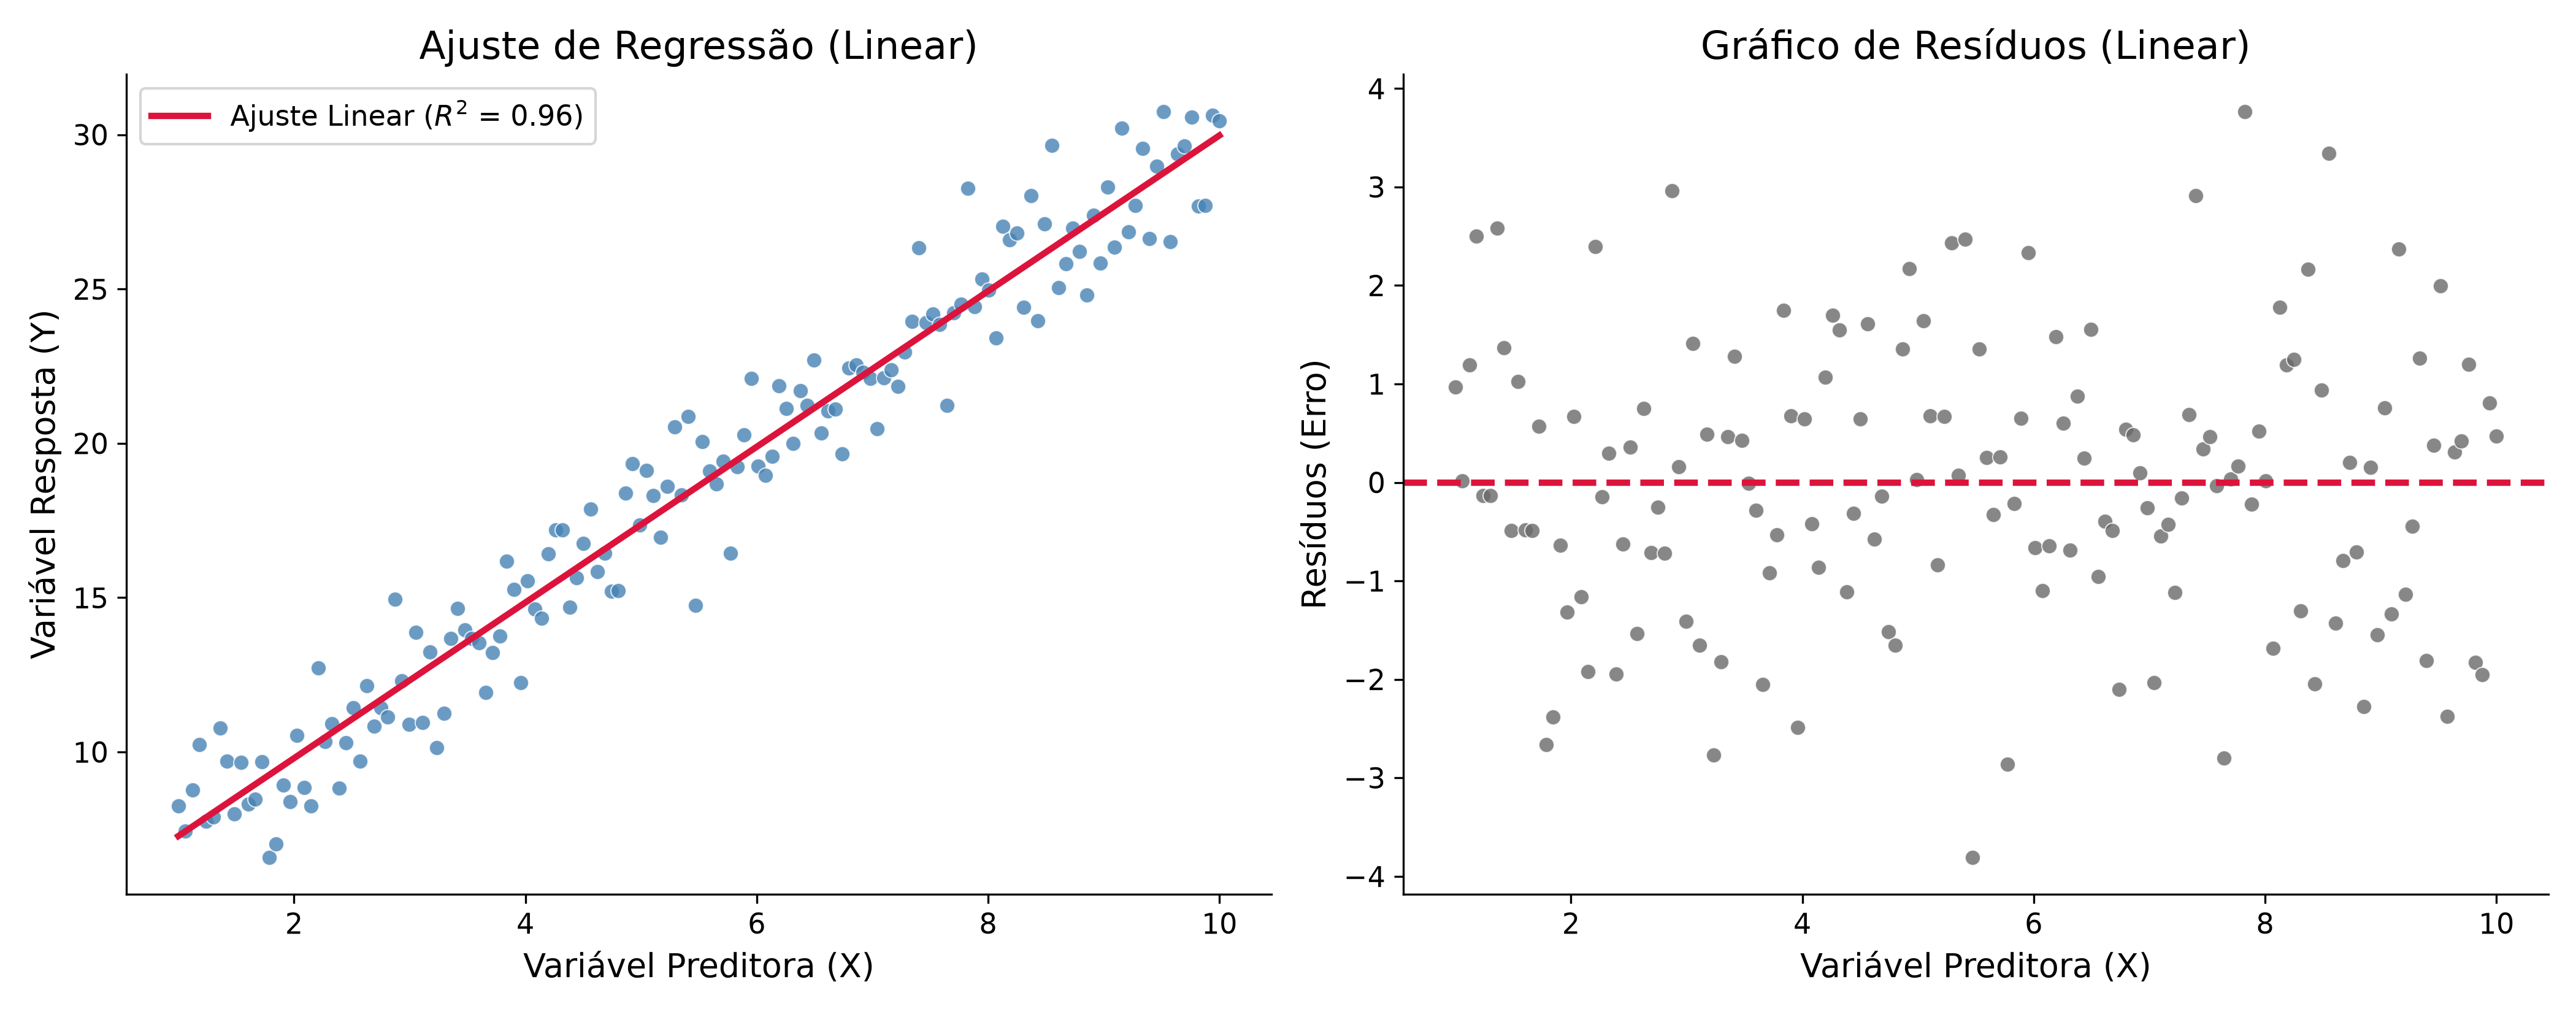
\includegraphics[width=\textwidth]{diagnostico_linear.png}
        \end{column}
    \end{columns}
\end{frame}

\begin{frame}{Diagnósticos Visuais: Não-Linearidade}
    \begin{columns}
        \begin{column}{0.5\textwidth}
            \textbf{Caso 2: Não-Linear}
            \begin{itemize}
                \item Os resíduos formam uma curvatura clara (formato em U ou padrão parabólico).
                \item Revela que a relação real entre $X$ e $Y$ não é linear.
                \item \textbf{Solução:} Requer transformações nas variáveis (ex: usar $\log(X)$) ou inclusão de termos polinomiais.
            \end{itemize}
        \end{column}
        \begin{column}{0.5\textwidth}
            \centering
            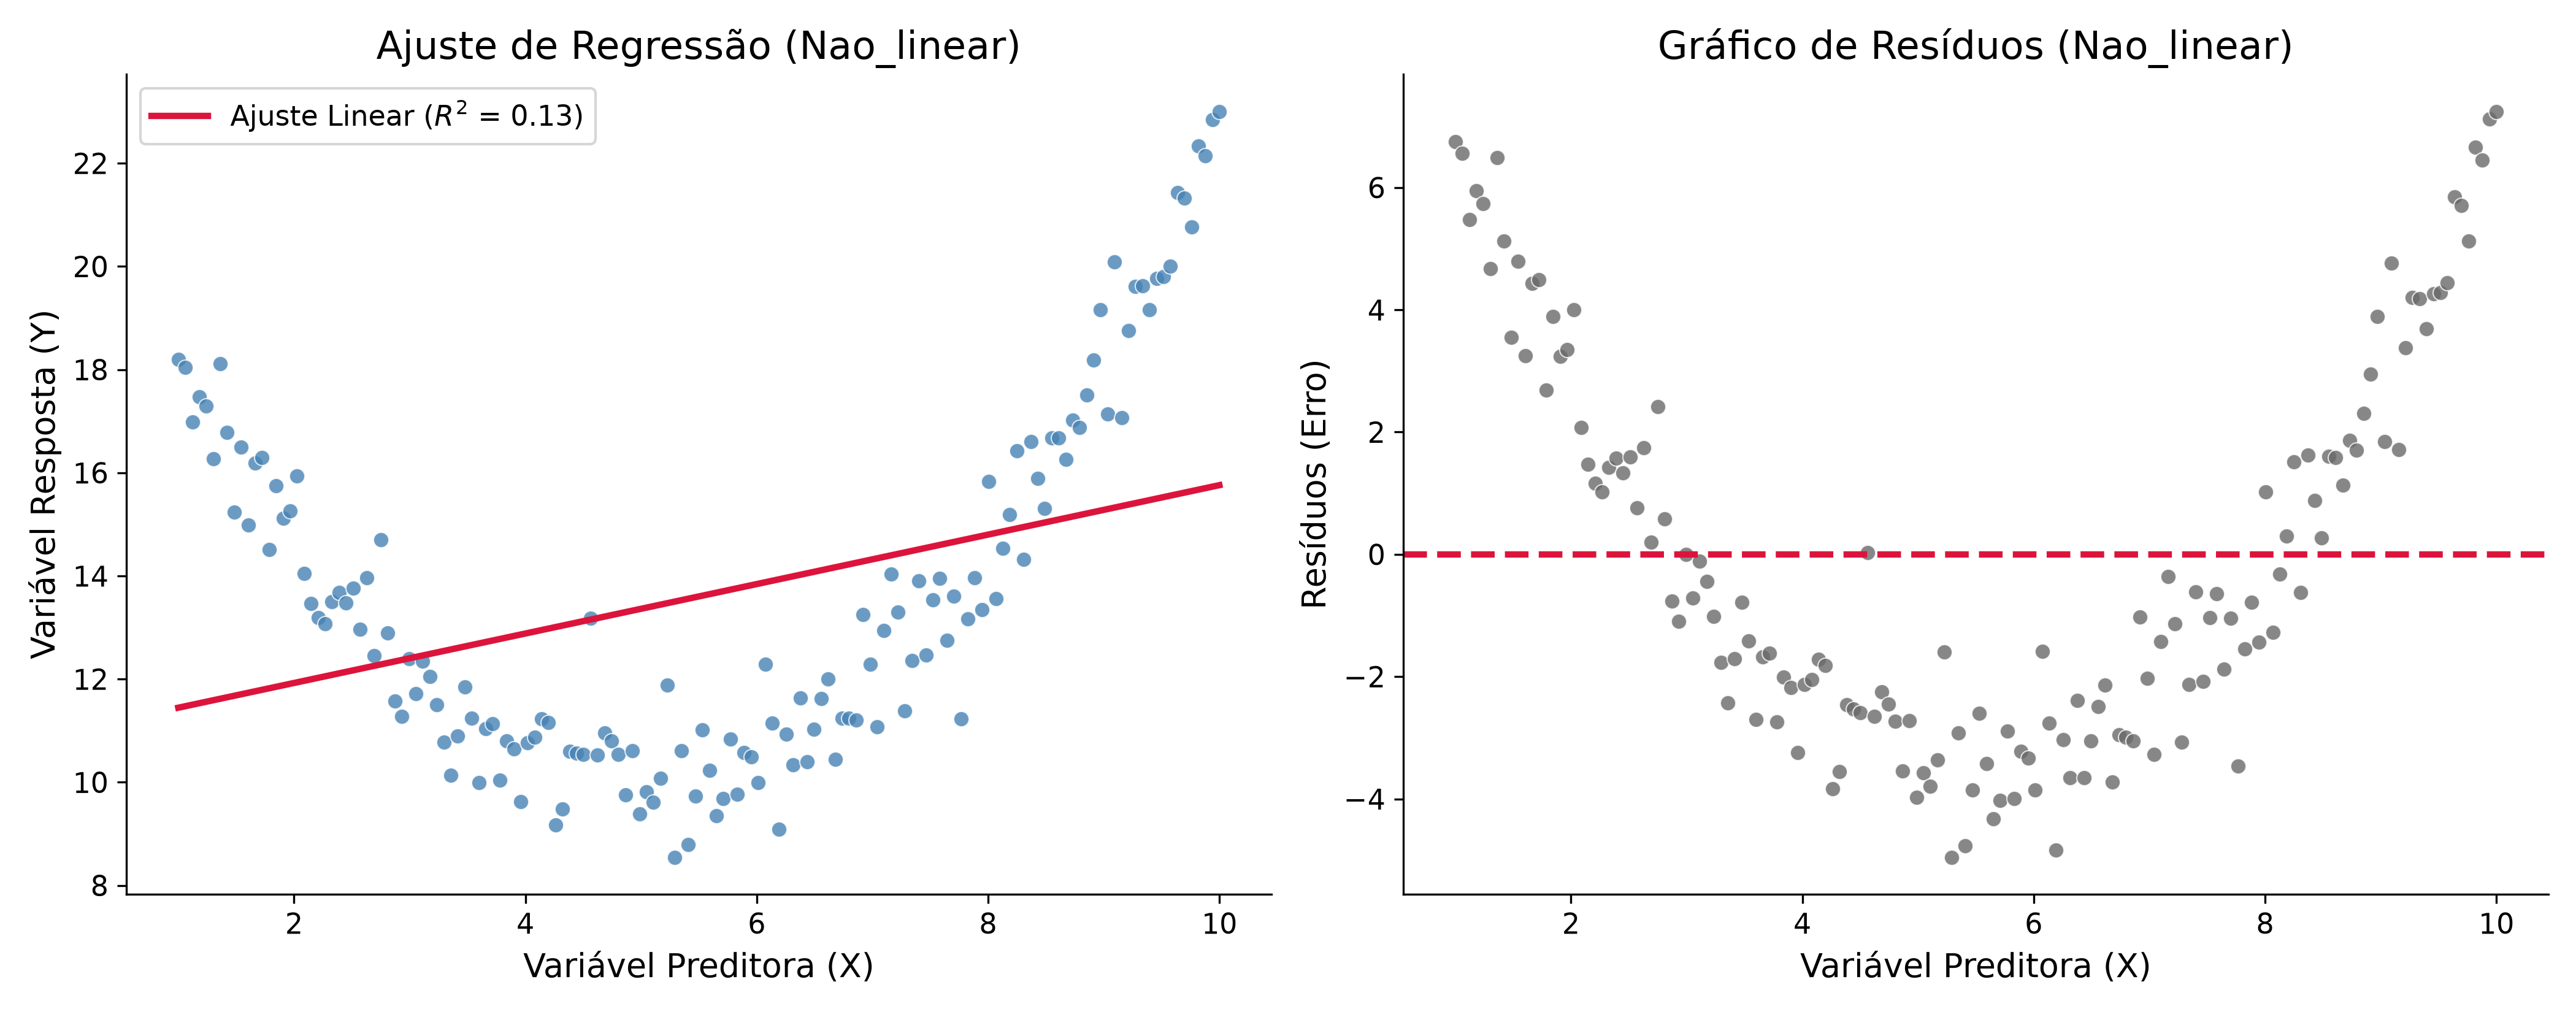
\includegraphics[width=\textwidth]{diagnostico_nao_linear.png}
        \end{column}
    \end{columns}
\end{frame}

\begin{frame}{Diagnósticos Visuais: Heterocedasticidade}
    \begin{columns}
        \begin{column}{0.5\textwidth}
            \textbf{Caso 3: Heterocedástico}
            \begin{itemize}
                \item A dispersão dos resíduos aumenta ou diminui sistematicamente à medida que $X$ cresce.
                \item Produz um padrão visual de "funil".
                \item \textbf{Consequência:} Invalida as fórmulas tradicionais de erro padrão do slope.
            \end{itemize}
        \end{column}
        \begin{column}{0.5\textwidth}
            \centering
            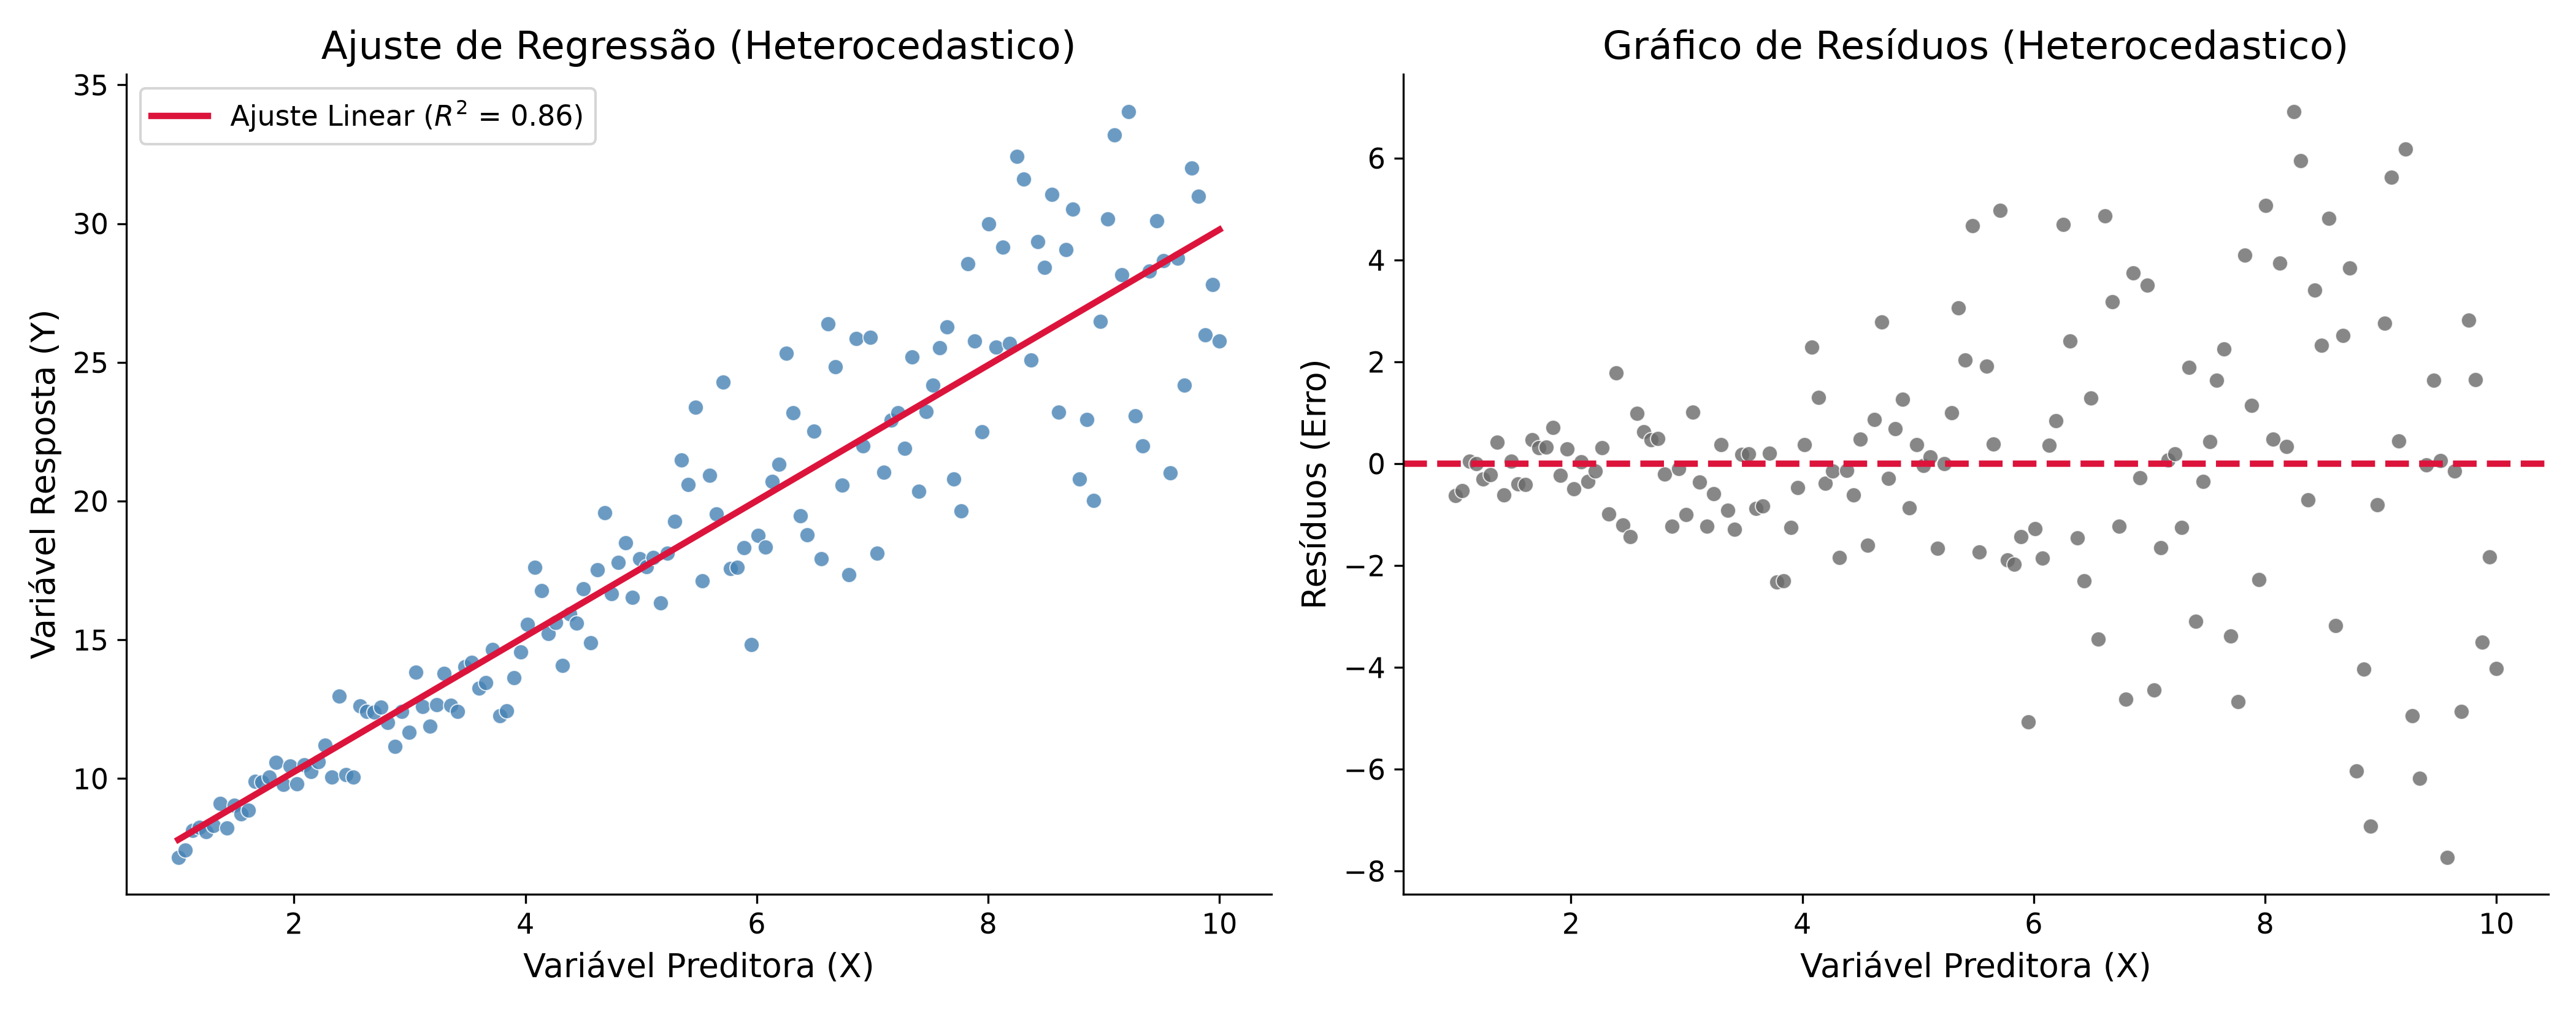
\includegraphics[width=\textwidth]{diagnostico_heterocedastico.png}
        \end{column}
    \end{columns}
\end{frame}

\begin{frame}{Diagnósticos Numéricos de Regressão}
    \begin{itemize}
        \item \textbf{Média dos Resíduos:} Na regressão de mínimos quadrados, a média amostral dos resíduos é matematicamente igual a zero:
        $$\bar{e} = \frac{1}{N} \sum_{i=1}^N e_i = 0$$
        \item \textbf{Desvio Padrão dos Resíduos} ($SD_{res}$): Mede o espalhamento vertical em torno da reta ajustada:
        $$SD_{res} = \sqrt{\frac{\sum e_i^2}{N - 2}} \approx \sqrt{1 - r^2} \cdot s_y$$
        \item Onde a aproximação teórica é dada pela multiplicação de $\sqrt{1 - r^2}$ pelo \textbf{Desvio Padrão Amostral} da variável resposta $s_y$.
    \end{itemize}
\end{frame}

\begin{frame}{Inferência do Slope por Reamostragem (Bootstrap)}
    \begin{itemize}
        \item Em conjuntos de dados amostrais, os coeficientes $\beta$ e $\alpha$ possuem incerteza estatística (erro padrão).
        \item Como construir um \textbf{Intervalo de Confiança} ($IC$) para o slope $\beta$ sem fazer suposições estritas de normalidade populacional?
        \item \textbf{Bootstrap de Pares:}
        \begin{enumerate}
            \item Sorteamos com reposição linhas completas da tabela amostral de tamanho $N$.
            \item Ajustamos uma reta para esta nova amostra Bootstrap e guardamos o slope $\beta_{boot}$.
            \item Repetimos o processo 2000 vezes para gerar a distribuição empírica do slope.
            \item Extraímos as posições 2.5\% e 97.5\% para formar o Intervalo de Confiança ($IC$) de 95\%.
        \end{enumerate}
    \end{itemize}
\end{frame}

\begin{frame}[fragile]{Exemplo Real: Comprimento e Cabeça de Gambás}
    \begin{block}{Comparação: Bootstrap vs. Statsmodels}
\begin{lstlisting}
import statsmodels.api as sm
import numpy as np

# X = comprimento do corpo (cm), Y = comprimento da cabeca (mm)
# Amostra simulada de 140 gambas
X_sm = sm.add_constant(comprimento_corpo)
modelo = sm.OLS(comprimento_cabeca, X_sm).fit()

print(modelo.summary().tables[1])
# Tabela classica reporta:
# const: coef = 42.6419 | IC 95% = [36.490, 48.794]
# x1:    coef = 0.5743 | IC 95% = [0.504,  0.644]

# Comparacao com Bootstrap de Pares:
# Slope estimado: 0.5743
# IC 95% Bootstrap: [0.5042, 0.6484]
\end{lstlisting}
    \end{block}
    \vspace{0.1cm}
    Os métodos concordam fortemente, validando o uso de ferramentas de simulação.
\end{frame}


\end{document}
